\documentclass[twocolumn,oneside,a4paper,10pt]{article}
\usepackage[english,brazilian]{babel}
\usepackage[alf]{abntex2cite}
\usepackage[utf8]{inputenc}
\usepackage[T1]{fontenc}
\usepackage[top=5mm, bottom=5mm, left=5mm, right=5mm]{geometry}
\usepackage{framed}
\usepackage{booktabs}
\usepackage{color}
\usepackage{hyperref}
\usepackage{graphicx}
\usepackage{float}
\graphicspath{{./Volumes/}}
%\usepackage{multicol}
\definecolor{shadecolor}{rgb}{0.8,0.8,0.8}

\newcommand{\EREM}{EREM Regina Pacis}
\newcommand{\curso}{\textbf{3 EMSI B}}
\newcommand{\professor}{Prof. Leandro Vieira}

\begin{document}
\pagestyle{empty}
análise de gráficos

\begin{center}
\EREM
\par %pula uma linha
\curso
\par
\professor
\par
\LARGE \textbf{Atividade de Matemática}
\end{center}

\begin{enumerate}

\item \textbf{(UCB - DF)}

\begin{figure}[!htb]
\center
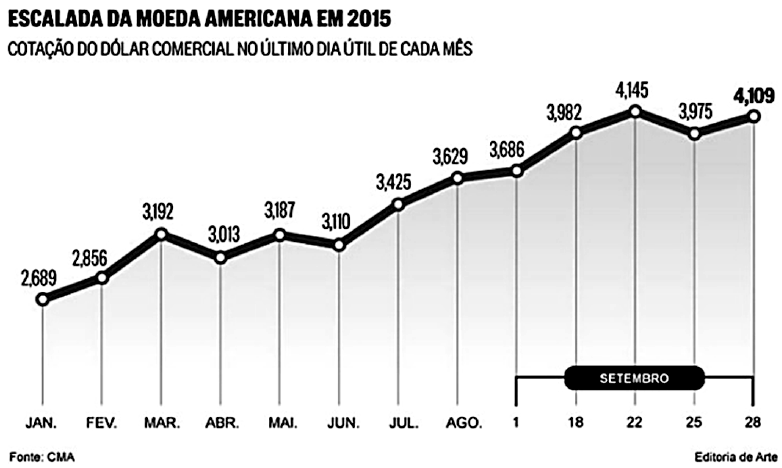
\includegraphics[width=8cm]{Figuras/g1.png}
\end{figure}

Com base exclusivamente nos dados apresentados no gráfico quanto à cotação do dólar comercial no último dia útil de cada mês de 2015, assinale a alternativa correta.

\begin{enumerate}
\item Em dezembro de 2014, a cotação do dólar comercial foi menor que 2,689.
\item O maior valor para a cotação do dólar comercial foi verificado em 28 de setembro.
\item A função que representa o valor da cotação do dólar comercial em relação ao tempo é crescente, no intervalo apresentado no gráfico.
\item A diferença entre os valores da cotação do dólar comercial de maio e de março foi menor que um centavo de real.
\item Em 15 de agosto, o valor da moeda foi menor que 3,629.
\end{enumerate}


\item \textbf{(UCB - DF)}

\begin{figure}[!htb]
\center
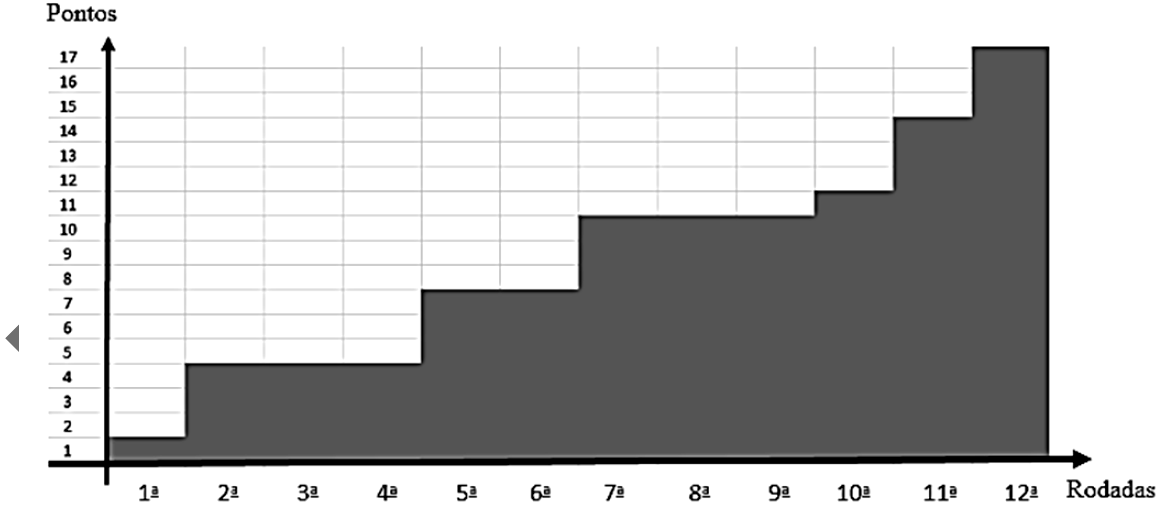
\includegraphics[width=8cm]{Figuras/g2.png}
\end{figure}

O gráfico mostra o número de pontos de uma equipe de futebol nas 12 primeiras rodadas de um campeonato. Sabendo que, nesse campeonato, em caso de vitória a equipe soma três pontos, em caso de empate soma um ponto e em caso de derrota não soma ponto, assinale a alternativa correta.

\begin{enumerate}
\item A equipe perdeu os jogos da segunda, terceira e quarta rodadas.
\item Nas doze rodadas, o número de vitórias foi igual ao número de derrotas.
\item A média de pontos obtidos por rodada, nessas doze rodadas, é igual a 1,5 pontos.
\item A equipe conseguiu dois empates entre a sétima e a nona rodadas.
\item Nas doze rodadas, a equipe empatou três vezes.
\end{enumerate}

\item O gráfico a seguir diz respeito aos resultados obtidos por uma turma de alunos de um curso preparatório específico para professor de educação básica.

\begin{figure}[!htb]
\center
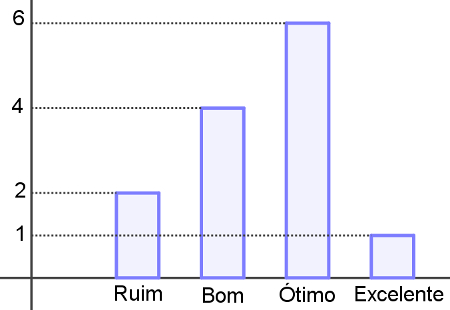
\includegraphics[width=6cm]{Figuras/g3.jpg}
\end{figure}

\newpage
Para continuar no mercado, é necessário que esse curso aprove pelo menos 70\% de seus alunos, que, por sua vez, são professores especializando-se. Sabendo que os aprovados são apenas aqueles que obtiveram resultado ótimo ou excelente, pode-se afirmar que esse curso continuará no mercado?

\begin{enumerate}
\item Sim, pois o percentual de professores aprovados foi, aproximadamente, 70\%
\item Sim, pois o percentual de professores aprovados foi, aproximadamente, 80\%
\item Não, pois o percentual de professores aprovados foi, aproximadamente, 50\%
\item Não, pois o percentual de professores aprovados foi, aproximadamente, 40\%
\item Sim, pois o percentual de professores aprovados foi, aproximadamente, 90\%
\end{enumerate}

O gráfico mostra o número de livros lidos por um estudante de 2014 a 2017.

\begin{figure}[!htb]
\center
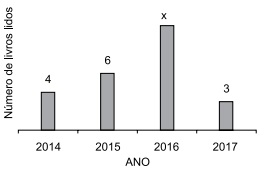
\includegraphics[width=6cm]{Figuras/m1.jpg}
\end{figure}

Considerando-se o número total de livros lidos nesses quatro anos, esse estudante leu, em média, 6 livros por ano. O número de livros lidos em 2016 foi

\begin{enumerate}
\item 7
\item 8
\item 9
\item 10
\item 11
\end{enumerate}

\item  O gráfico a seguir apresenta a quantidade de alunos de uma escola que praticam cada um dos seguintes esportes: vôlei, handball, futebol e judô. Apresenta também a quantidade de homens e mulheres que praticam cada uma das atividades.

\begin{figure}[!htb]
\center
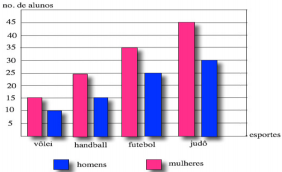
\includegraphics[width=5cm]{Figuras/g4.png}
\end{figure}

De acordo com os dados apresentados no gráfico acima, qual a alternativa correta?

\begin{enumerate}
\item Aproximadamente 80\% dos alunos jogam handball.
\item Dentre os que jogam futebol, 25\% são homens.
\item 40\% dos alunos são homens.
\item Dentre os alunos que são mulheres, 45\% lutam judô.
\item A diferença entre o número de mulheres e homens corresponde a 40\% dos alunos.

\end{enumerate}

\item

Para ter uma conta em banco, o brasileiro paga uma tarifa mensal que lhe dá acesso a um determinado pacote de serviços. O gráfico de setores, resultado de um levantamento feito com usuários dos cinco maiores bancos do País, mostra a distribuição percentual dos valores mensais pagos.

\begin{figure}[!htb]
\center
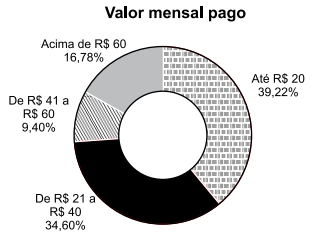
\includegraphics[width=5cm]{Figuras/g5.png}
\end{figure}

\newpage
Se 40 920 usuários afirmaram que pagam mensalmente valores que vão de R\$ 21,00 até R\$ 60,00, então o número total de pessoas ouvidas nesse levantamento foi igual a

\begin{enumerate}
\item 93 000.
\item 92 500.
\item 90 000.
\item 88 800.
\item 79 000.
\end{enumerate}

\item O gráfico a seguir mostra o número de tablets vendidos no Brasil, em milhares de unidades, no período de 2010 a 2015.

\begin{figure}[!htb]
\center
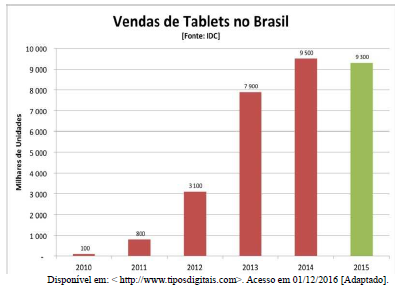
\includegraphics[width=7cm]{Figuras/g6.png}
\end{figure}


Considere que o número de tablets vendidos no Brasil, em 2016, foi igual à média aritmética do número de tablets vendidos nos últimos três anos apresentados no gráfico. Então, o número de tablets vendidos no Brasil, em 2016, em milhares de unidades, foi igual a

\begin{enumerate}
\item 8900
\item 9400
\item 13350
\item 26700
\end{enumerate}

\item Aqui vai um teste.

\item Mais outro test.

\item O gráfico a seguir mostra o número de contratos do Fies no Brasil, em mil unidades, no período de 2010 a 2018.

\begin{figure}[!htb]
\center
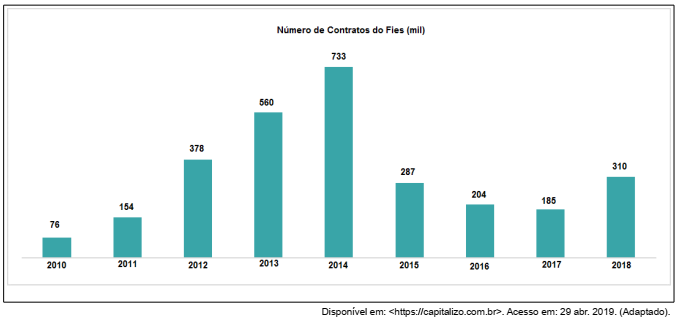
\includegraphics[width=5cm]{Figuras/g7.png}
\end{figure}

De acordo com os dados apresentados, o período que apresentou a maior taxa de crescimento foi em
\begin{enumerate}
\item 2010/2011
\item 2011/2012
\item 2013/2014
\item 2014/2015
\end{enumerate}


\item  \textbf{(BB – Fundação Carlos Chagas)} O supervisor de uma agência bancária obteve dois gráficos que mostravam o número de atendimentos realizados por funcionários. O Gráfico I mostra o número de atendimentos realizados pelos funcionários A e B, durante 2 horas e meia, e o Gráfico II mostra o número de atendimentos realizados pelos funcionários C, D e E, durante 3 horas e meia.

\newpage
\begin{figure}[!htb]
\center
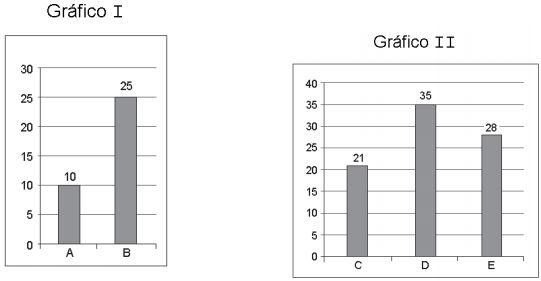
\includegraphics[width=9cm]{Figuras/g9.jpg}
\end{figure}

Observando os dois gráficos, o supervisor desses funcionários calculou o número de atendimentos, por hora, que cada um deles executou. O número de atendimentos, por hora, que o funcionário B realizou a mais que o funcionário C é:
\begin{enumerate}
\item 4
\item 3
\item 10
\item 5
\item 6
\end{enumerate}

\item \textbf{(PM Pará)} O gráfico abaixo mostra a produção diária de lixo orgânico de duas pessoas. O dia da semana que o gráfico mostra que as produções de lixo das duas pessoas foram iguais é:

\begin{figure}[!htb]
\center
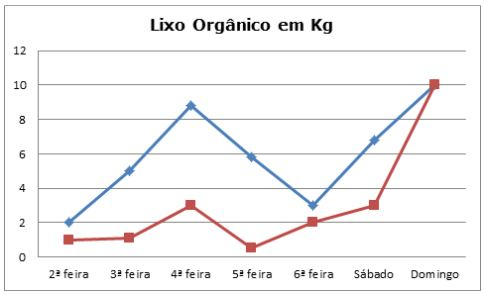
\includegraphics[width=8cm]{Figuras/g10.jpg}
\end{figure}

\begin{enumerate}
\item 2ª feira
\item 4ª feira
\item 6ª feira
\item Sábado
\item Domingo
\end{enumerate}

\item \textbf{ENEM} O dono de uma farmácia resolveu colocar à vista do público o gráfico mostrado a seguir, que apresenta a evolução do total de vendas (em reais) de certo medicamento ao longo do ano de 2011.

\begin{figure}[!htb]
\center
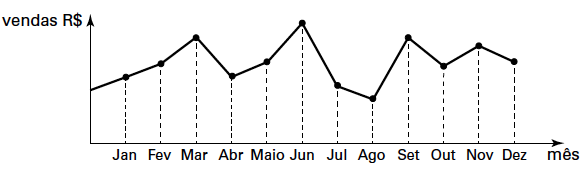
\includegraphics[width=6cm]{Figuras/g11.png}
\end{figure}

De acordo com o gráfico, os meses em que ocorreram, respectivamente, a maior e a menor venda absolutas em 2011 foram

\begin{enumerate}
\item março e abril.
\item março e agosto.
\item agosto e setembro.
\item junho e setembro.
\item junho e agosto.
\end{enumerate}

\newpage
\item \textbf{ENEM} O gráfico expõe alguns números da gripe A-H1N1. Entre as categorias que estão em processo de imunização, uma já está completamente imunizada, a dos trabalhadores da saúde.

\begin{figure}[!htb]
\center
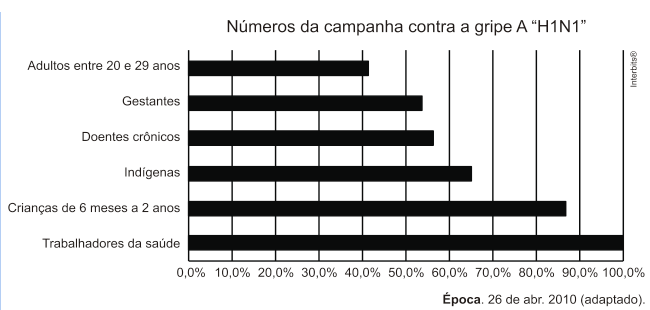
\includegraphics[width=8cm]{Figuras/g12.png}
\end{figure}

De acordo com o gráfico, entre as demais categorias, a que está mais exposta ao vírus da gripe A-H1N1 é a categoria de

\begin{enumerate}
\item indígenas.
\item gestantes.
\item doentes crônicos.
\item adultos entre 20 e 29 anos.
\item crianças de 6 meses a 2 anos.
\end{enumerate}

\item A distribuição dos salários dos 200 funcionários, em R\$ 1.000,00, de determinada carreira profissional em um órgão público está representada pelo histograma abaixo. No eixo vertical estão assinaladas as respectivas densidades de frequências, em (R\$ 1.000,00)-1. Define-se densidade de frequência de um intervalo de classe como sendo o quociente da divisão da respectiva frequência relativa pela correspondente amplitude do intervalo.

\begin{figure}[!htb]
\center
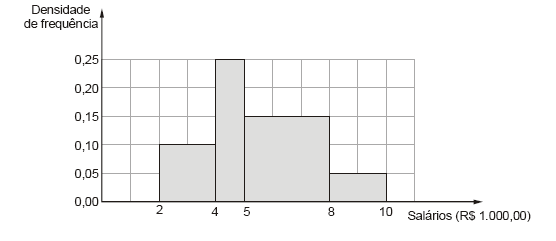
\includegraphics[width=8cm]{Figuras/g13.png}
\end{figure}

Considerando todos os intervalos de classe fechados à esquerda e abertos à direita, tem-se que a quantidade de funcionários que possuem salários maiores ou iguais a R\$ 4.000,00 e inferiores a R\$ 8.000,00 é

\begin{enumerate}
\item 60
\item 80
\item 90
\item 140
\item 160
\end{enumerate}

\item Em um blog de variedades, músicas, mantras e informações diversas, foram postados “Contos de Halloween”. Após a leitura, os visitantes poderiam opinar, assinalando suas reações em: “Divertido”, “Assustador” ou “Chato”. Ao final de uma semana, o blog registrou que 500 visitantes distintos acessaram esta postagem. O gráfico a seguir apresenta o resultado da enquete.

\begin{figure}[!htb]
\center
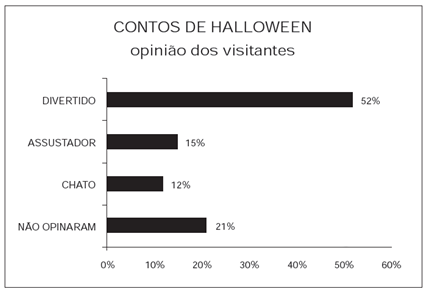
\includegraphics[width=8cm]{Figuras/h1.png}
\end{figure}
\newpage
O administrador do blog irá sortear um livro entre os visitantes que opinaram na postagem “Contos de Halloween”. Sabendo que nenhum visitante votou mais de uma vez, a probabilidade de uma pessoa escolhida ao acaso entre as que opinaram ter assinalado que o conto “Contos de Halloween” é “Chato” é mais aproximada por:

\begin{enumerate}
    \item 0,09.
    \item 0,12.
   	\item 0,14.
    \item 0,15.
    \item 0,18.
\end{enumerate}

\item Os dados da tabela a seguir fornecem resultados de uma pesquisa social de renda e satisfação no trabalho nos Estados Unidos (Agresti, 1990, p. 21) e foram retirados do livro: Lindsey, J. K. (1994) Introductory Statistics: A Modelling Approach. Oxford Science Publications.

\begin{figure}[!htb]
\center
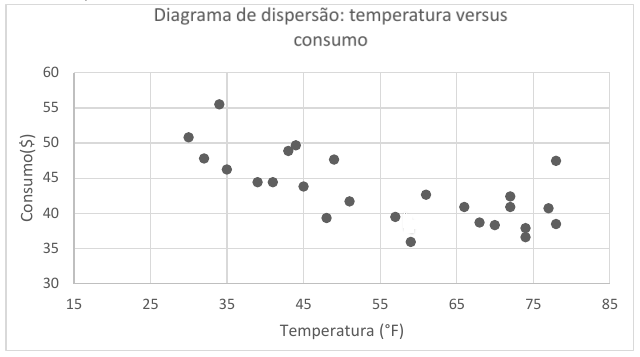
\includegraphics[width=8cm]{Figuras/g14.png}
\end{figure}

Na tabela são apresentadas as respostas de 801 pessoas que participaram da pesquisa sobre a sua satisfação em relação ao seu trabalho (muito insatisfeito, pouco insatisfeito, moderadamente satisfeito, muito satisfeito) e renda. Com base nas informações apresentadas, responda aos seguintes ítens:
	\begin{enumerate}
	\item Qual o percentual das pessoas pesquisadas que tem um redimento na faixa salarial de 6000 a 14999:
	\item Qual o percentual de pessoas pesquisadas que estão muito insatisfeitas:
	\item Qual a diferença entre o percentual de pessoas muito satisfeitos entre o que as pessoas que recebem o salário na maior faixa salarial e menor faixa salarial:
	\item Dentre os pequisados que recebem salários inferiores a 6000, qual o percentual daqueles que são moderadamente satisfeitos com o seu trabalho:
	\end{enumerate}

\item O figura a seguir apresenta dados sobre a temperatura em graus Fahrenheit e o consumo de energia (em dólares) de uma residência no hemisfério norte entre os meses de abril de 1991 e julho de 1993.

\begin{figure}[!htb]
\center
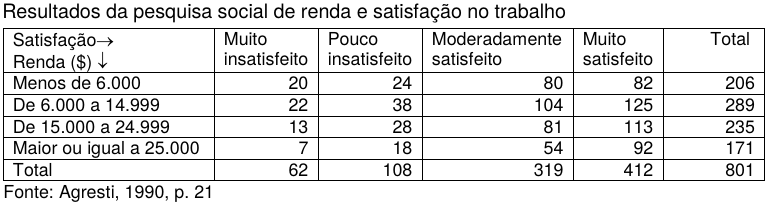
\includegraphics[width=8cm]{Figuras/g15.png}
\end{figure}

Com base nas informações apresentadas, julgue os ítens a seguir em verdadeiro ou falso:
\begin{enumerate}
	\item O maior valor
	\item Analisando o diagrama de dispersão da fig10ura podemos perceber uma tendência de quanto maior a temperatura, menor é o consumo de energia.
\end{enumerate}

\end{enumerate}

\vspace{80pt}
\flushbottom
\flushright
"A arte de viver é simplesmente a arte de conviver...\\Simplesmente, disse eu? Mas como é difícil!\\(Mario Quintana)

\end{document}
